% 图像坐标系
% 图像|像素|坐标系

下面介绍的这种坐标在图片处理中广泛使用(例如 Matlab 也采用这种定义\footnote{见 \lstinline|imshow|, \lstinline|ginput| 等函数}).

如\autoref{imgFrm_fig1}, 图片中每个像素可以表示为一个正方形, 我们 $x$ 方向指向右, $y$ 方向指向下, 令左上角的像素的正方形中心坐标为 $(1, 1)$, 所以坐标原点和坐标轴落在图片外面.

\begin{figure}[ht]
\centering
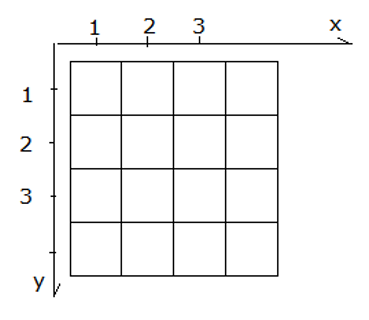
\includegraphics[width=5cm]{./figures/imgFrm_1.png}
\caption{图片坐标系} \label{imgFrm_fig1}
\end{figure}
